\section{Introduction}
\label{sec:intro}

Audio tagging is the task to label the sound recordings with representative tags like sound events. It can be used in many applications like music tagging \citep{fu2010survey}, sound retrieval \citep{font2018sound} and urban sound planning \citep{bello2019sonyc}. However, the manual labeling required by a well-performing tagging model can be heavy and expensive. Compared to annotating for images classification, annotators have to spend substantially more time on finishing the whole recording before tagging. Consequently, even the largest dataset for audio tagging, AudioSet \citep{gemmeke2017audio}, is orders of magnitude smaller than image classification datasets \citep{deng2009imagenet, thomee2016yfcc100m}, and many other common datasets are even smaller, like SONYC \citep{bello2019sonyc} with only 2,351 training recordings. Therefore, when we want to tailor a new dataset for particular needs, the data size tends to be limited, and thus robust methods in such low-resource scenarios are largely desired.

Structured knowledge has been shown effective in the low-resource setting of many tasks \citep{shwartz2020unsupervised, feng2020scalable, ji2020language, li2013data, zhang2013automatic}, while the exploration of knowledge is still limited for audio tagging. These works mainly focus on ontological knowledge \citep{jati2019hierarchy, sun2020ontology, shrivaslava2020mt}. For example, AudioSet involves \textit{IsA} relations between sound events, such as \textit{Speech IsA Human voice}. Models enhanced with such knowledge can effectively capture the similarity between tags of similar category. However, ontological knowledge failed to cover other relations between different categories, like the frequent \textit{Co-occurrence} of \textit{Car} sounds and \textit{Engine} sounds. Such relationships are still under-explored.

\begin{figure}[htbp]
  \setlength{\abovecaptionskip}{0.cm}
\setlength{\belowcaptionskip}{-0.5cm}
  \centering
  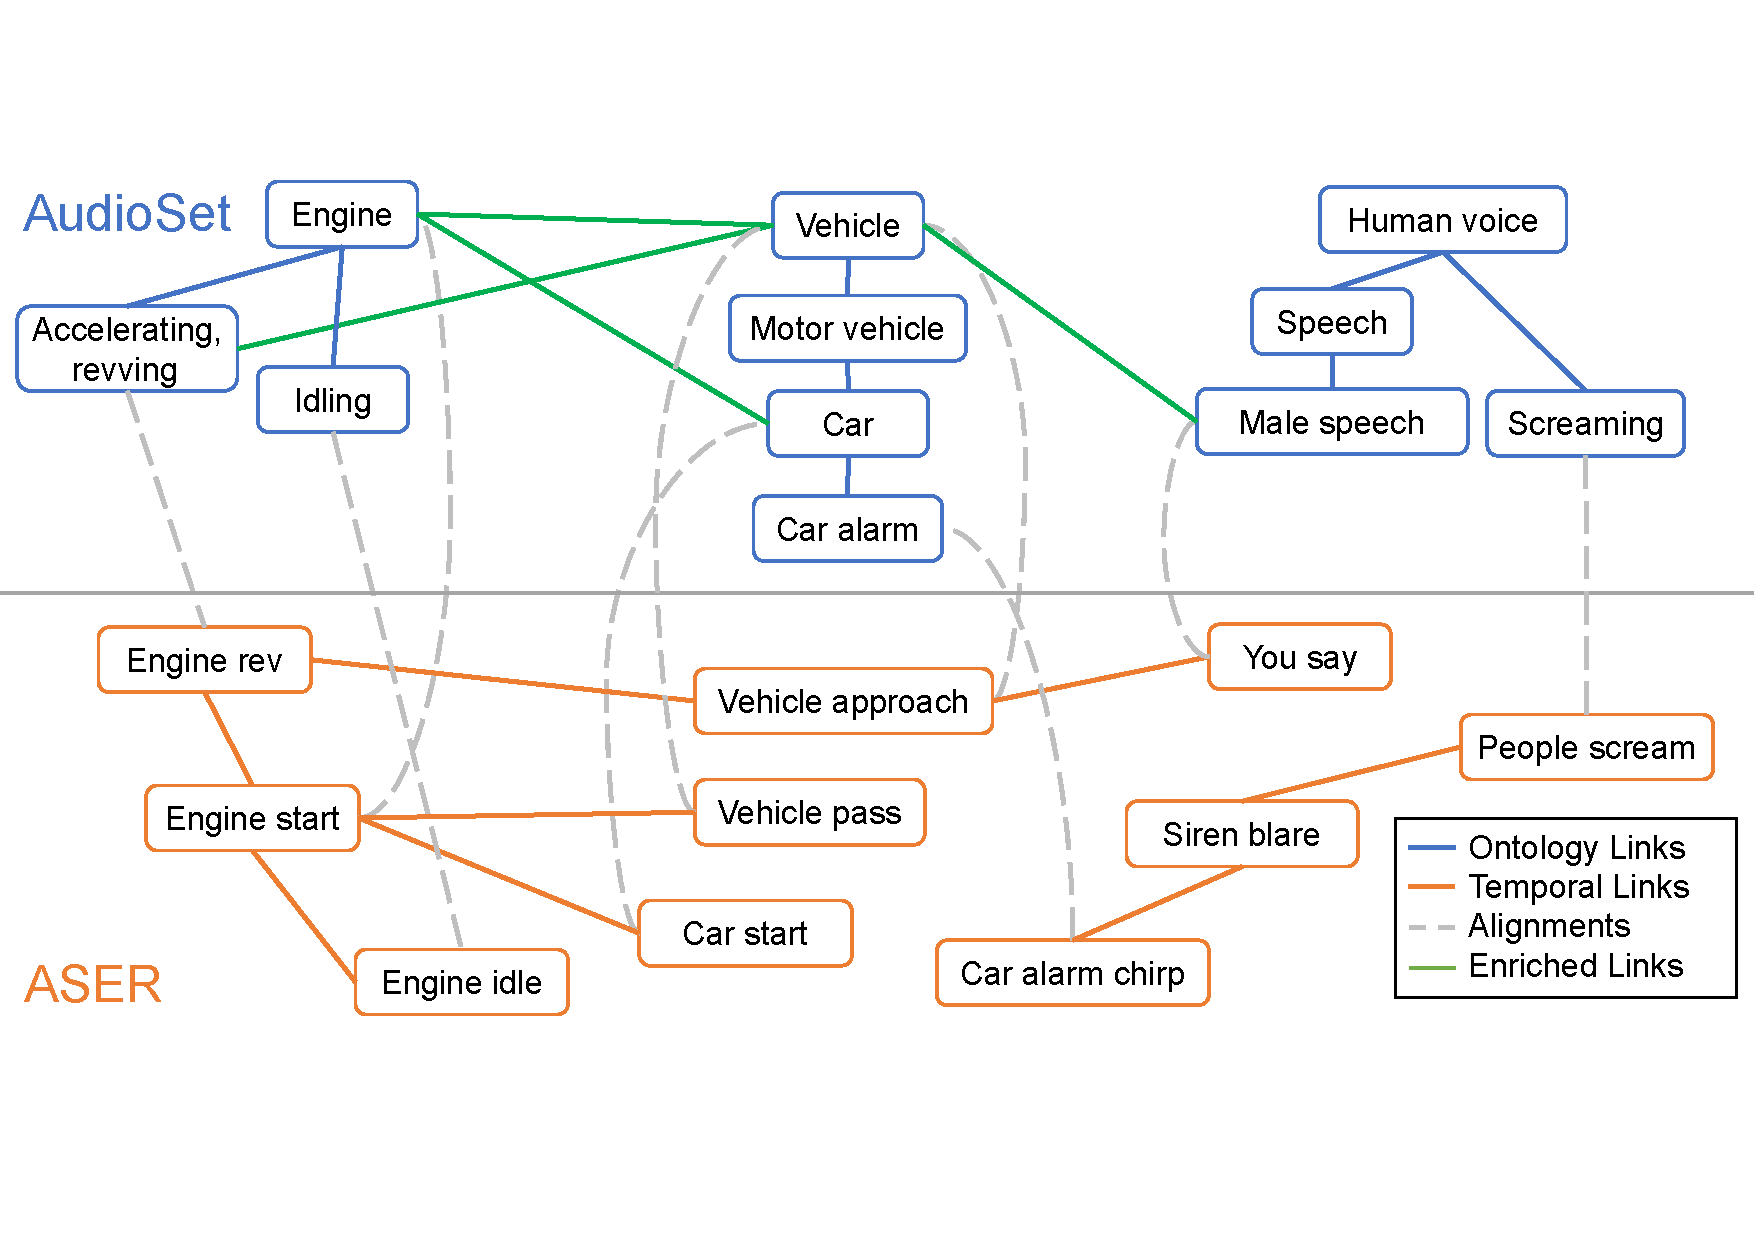
\includegraphics[width=\linewidth]{figures/align1.pdf}
  \caption{Aligning ASER to AudioSet. We establish an enriched link between two AudioSet events if their corresponding ASER events have temporal links.}
  \label{fig:align}
\end{figure}

To extend the dimensions of available knowledge for audio analysis, 
we propose to construct temporal knowledge graph on top of pre-defined audio tags 
with the knowledge transferred from ASER \citep{zhang2020aser}, 
a large-scale commonsense knowledge graph about the relations between events extracted 
from textual corpus. Here we pay special attention to temporal relations 
like \textit{Precedence} and \textit{Conjunction}, 
which we will collectively refer to as ``temporal links''.
They can provide hints whether 2 events might co-occur in a short period, 
as is the case for multi-label audio tagging. 
This kind of knowledge is similar to the sound event co-occurrence graph mined 
from audio dataset \citep{shrivaslava2020mt, wang2020modeling} to some extent, 
but they come from different sources, i.e., text vs. audio. 
Algorithms to mine sound event co-occurrence from audio data
rely on dataset-specific hyperparameter tuning, 
and large-scale, accurate, multi-label annotations, 
which can be hard to obtain due to missing labels problems~\citep{fonseca2020addressing},
or from single-label or low-resource datasets.

The knowledge construction requires the alignments between ASER events and domain-specific 
label sets, usually accompanied with ontologies, such as AudioSet (\figref{fig:align}).
We will then add an enriched link between two Audioset events if any pair of their aligned events in ASER have temporal links.
There are many challenges in establishing the alignments. 
First, there are mismatches between the event representations. For example, 
events are usually named with representative noun phrases or verb phrases in AudioSet, 
while ASER provides a finer representation of short clauses. 
Therefore, one AudioSet event can be aligned to multiple related ASER events, 
like \textit{Vehicle} to \textit{Vehicle approach} and \textit{Vehicle pass}. 
Moreover, the alignments should be decided according to acoustic relatedness rather 
than lexical or semantical similarity alone. For instance, we should not 
treat \textit{I see engine} as related to the sound event of \textit{Engine} 
despite the shared object, as the former event doesn't make a sound. In contrast, 
we should link \textit{Male Speech} to \textit{You say} although they have no words
in common.

In this work, we propose a semi-automatic approach to align the events in ASER and those in
the target label set. We use heuristics to automatically extract audible events in
ASER that are synonymous to those events in AudioSet, with the help of Word Sense Disambiguation (WSD) \citep{lesk1986automatic} and WordNet \citep{miller1995wordnet}. For AudioSet, candidate alignments are also verified
manually to ensure the quality of final temporal KG.
%Initially, to alleviate the lexical differences between the two event representations, 
%we apply preprocessing to the original sound event labels to match the lemmatized representation of ASER, and expansion to produce queries that can cover the various possible expressions 
%of acoustically related events. Next, these queries are sent to an information retrieval 
%system to fetch potentially related events from ASER. 
%These events then serve as candidate for alignments, and currently we will either manually 
%select or using some heuristics to eliminate the false candidates. 
%Finally, the remaining events and the relations between them can be aligned to the 
%original label set. 
% The resulting temporal KGs can be directly incorporated into existing 
% Graph Convolutional Network(GCN)-based models, and we propose a variant called Double-GCN (D
% -GCN) to combine the strength of ontological and temporal knowledge. 
The resulting temporal KGs can be directly incorporated into existing Graph Convolutional Network (GCN)-based models. We conduct experiments on two audio tagging datasets in different domains: the open domain AudioSet \citep{gemmeke2017audio} and SONYC urban sound tagging dataset \citep{bello2019sonyc}. Results suggest the usefulness of temporal knowledge in low resource settings. Nonetheless, simple combination of temporal and ontological knowledge sources in one graph doesn't provide performance gain. We hypothesize that a single graph can't model the heterogeneity of the two knowledge types properly. Inspired by R-GCN \citep{schlichtkrull2018modeling}, we further propose D-GCN that applies relation-specific transformation for two knowledge types.

In summary, our contributions are: 
(1) We propose a semi-automatic approach to construct temporal commonsense knowledge graph to enrich different audio tagging ontologies like AudioSet and SONYC.
(2) We propose to use a variant of R-GCN of two relation types, D-GCN, 
to leverage the heterogeneity of ontological and temporal knowledge.
(3) Experiments on AudioSet and SONYC dataset in low-resource settings show 
that temporal KG-enhanced model outperforms backbone model without KG, and 
combining ontology and temporal KG with D-GCN can provide further improvement. \footnote{Code and data: \url{https://github.com/blmoistawinde/dgcn_tagging}}


